\section{Red Despegar}

Para este experimento se tomo una captura de 20 minutos de la red por cable de despegar.com.

\begin{figure}[h]
  \centering
    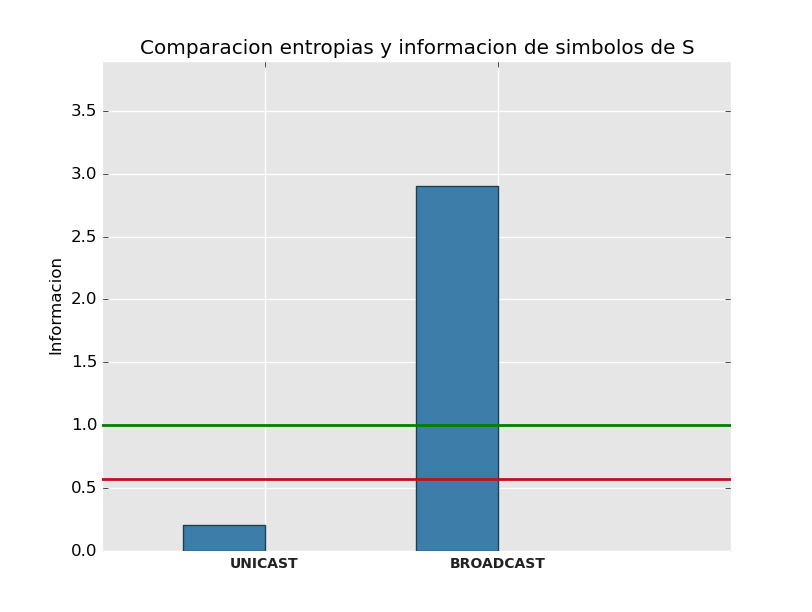
\includegraphics[width=0.45\textwidth]{entropia_red_despegar_s.png}
  \caption{Entropia de la fuente}
  \label{entropia-s}
\end{figure}

Como podemos ver en el gráfico comparativo la entropía no llega a ser máxima. De hecho puede verse en el símbolo $BROADCAST$ proporciona mucha mas información que el símbolo $UNICAST$. 

Por lo que hay un mayor flujo de paquetes Ethernet $UNICAST$ que $BROADCAST$, esto podría deberse a cambios en la topología de la red.


    \begin{table}[ht]\begin{center}
      \begin{tabular}{|c|c|}
      \hline
      \textbf{Nodo} & \textbf{Información} \\ \hline
      \texttt{UNICAST}& 0.207536 \\ \hline
      \texttt{BROADCAST}& 2.899857 \\ \hline
      \end{tabular}
      \caption{Información de los símbolos de S}
      \label{info-simbolos}
    \end{center}\end{table}

La entropia de la fuente da $0.568266518529$ mucho  menor que la maxima entropia que es $1$

El overhead impuesto por la red influencia la entropía de esta fuente.
Por ejemplo, si hubiese mas mensajes $ARP$ $BROADCAST$ la información del símbolo $S_{BROADCAST}$ bajaría haciendo consecuentemente que la entropía de la fuente $S$ se vea modificada.

\begin{figure}[h]
  \centering
    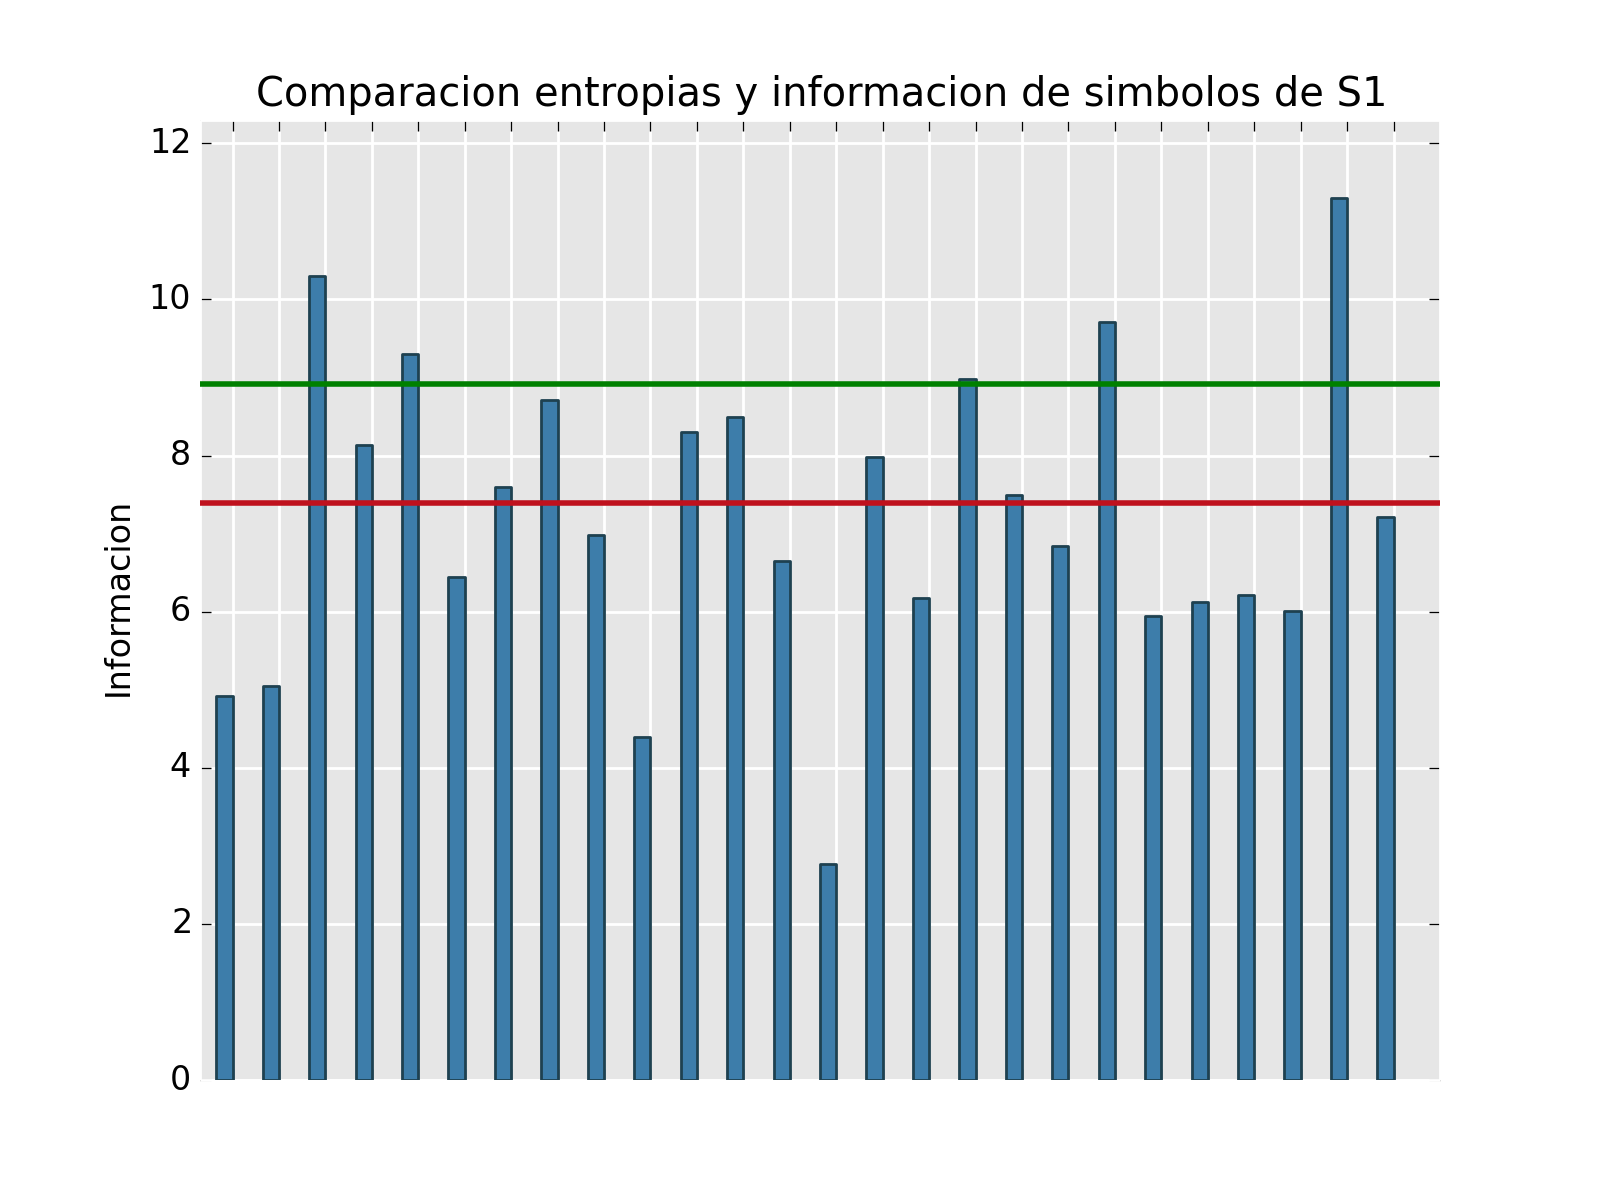
\includegraphics[width=0.45\textwidth]{entropia_red_despegar.png}
  \caption{Entropia de la fuente}
  \label{entropia-s1}
\end{figure}
En este gráfico agrupamos la información puesto que había demasiados símbolos.

En comparación con el resto de los mensajes el tráfico $ARP$ es bajo, el total de paquetes ethernet es $77755$, mientras que los paquetes $ARP$ son $2520$ sólo el 3\%, lo cual indica aparentemente que las tablas que mantienen la información de $ARP$ estan con informacion correcta. 
\\En base al criterio propuesto, se pueden distinguir 16 nodos, que en el grafico se corresponden con las 16 barras que están por debajo de la entroppía de la fuente:   

    \begin{table}[ht]\begin{center}
      \begin{tabular}{|c|c|}
      \hline
      \textbf{Nodo} & \textbf{Informacion} \\ \hline
      \texttt{10.254.213.254}&2.771731\\ \hline
      \texttt{10.254.213.74}&4.392317\\ \hline
      \texttt{10.254.213.103}&4.924169\\ \hline
      \texttt{10.254.95.254}&5.051281 \\ \hline
      \texttt{10.254.213.95}&5.941656 \\ \hline
      \texttt{10.254.213.63}&6.013806 \\ \hline
      \texttt{10.254.213.6}&6.129283 \\ \hline
      \texttt{10.254.213.37}&6.169925 \\ \hline
      \texttt{10.254.213.18}&6.169925 \\ \hline
      \texttt{10.254.213.13}&6.211745 \\ \hline
      \end{tabular}
      \caption{Nodos destacados}
      \label{Nodos-destacados}
    \end{center}\end{table}

Como en nuestra fuente estamos tomando las IPs destino de los paquetes $ARP$ $Who-has$. Esto indíca que estas IPs son muy frecuentes con lo cual se podría pensar en el escenario en que la mayoría de los nodos quiere conocer la MAC del Default Gateway por lo tanto envían tramas $Who-has$ con la dirección destino del mismo.


\begin{figure}[h]
  \centering
    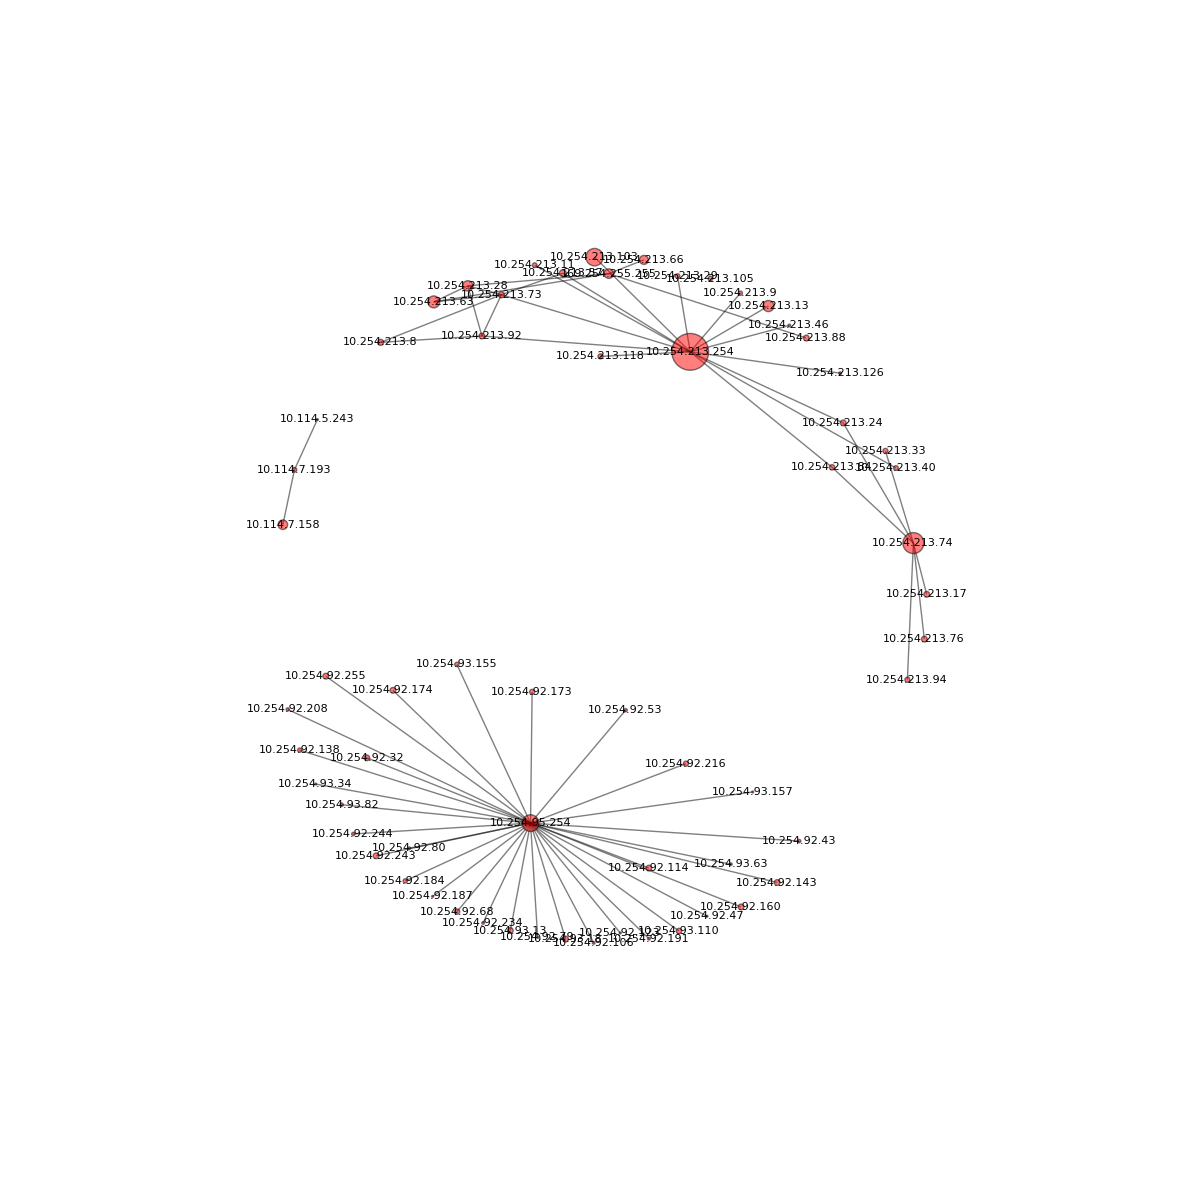
\includegraphics[width=0.45\textwidth]{grafo_red_despegar.png}
  \caption{Grafo de la fuente S1}
  \label{grafo-s1}
\end{figure}